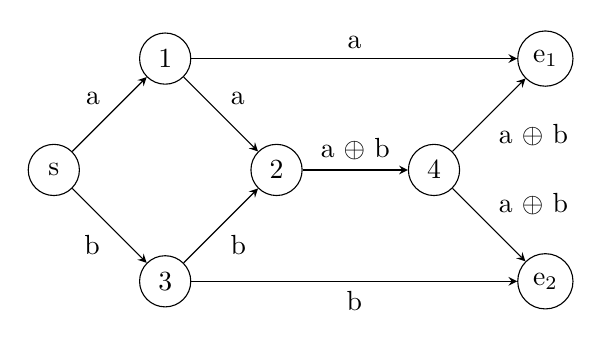
\begin{tikzpicture}[->,>=stealth,node distance=2cm,
	main/.style={shape=circle, draw=black, minimum size=6.5mm},
	empty/.style={}];
	\node[main] (1) [] {s};
	\node[main] (2) [above right of=1] {1};
	\node[main] (3) [below right of=2] {2};
	\node[main] (4) [below right of=1] {3};
	
	\node[main] (5) [right of=3,] {4};
	\node[main] (6) [above right of=5] {e\textsubscript{1}};
	\node[main] (7) [below right of=5] {e\textsubscript{2}};
	
	\path
	(1) edge node [above left] {a} (2)
	(1) edge node [below left] {b} (4)
	(2) edge node [above right] {a} (3)
	(4) edge node [below right] {b} (3)
	(3) edge node [above] {a $\oplus$ b} (5)
	(5) edge node [below right] {a $\oplus$ b} (6)
	(5) edge node [above right] {a $\oplus$ b} (7)
	(2) edge node [above] {a} (6)
	(4) edge node [below] {b} (7);
\end{tikzpicture}